%!TEX program = xelatex

\documentclass[a4paper, openany, oneside]{memoir}
\usepackage[no-math]{fontspec}
\usepackage{pgfplots}
\usepackage{float}
\pgfplotsset{compat=newest}
\usepackage{commath}
\usepackage{mathtools}
\usepackage{amssymb}
\usepackage{amsthm}
\usepackage{booktabs}
\usepackage{todonotes}
\usepackage{mathtools}
\usepackage{xcolor}
\usepackage[separate-uncertainty=true, per-mode=symbol]{siunitx}
\usepackage{listings}
\usepackage[american inductor, european resistor]{circuitikz}
\usepackage{amsmath}
\usepackage{amsfonts}
\usepackage{ifxetex}
\usepackage[dutch,english]{babel}
\usepackage[backend=bibtexu,texencoding=utf8,bibencoding=utf8,style=ieee,sortlocale=en_GB,language=auto]{biblatex}
\usepackage[strict,autostyle]{csquotes}
\usepackage{import}
\usepackage{standalone}
\usepackage{bookmark,hyperref}
\usepackage{xcolor,mdframed}
\usepackage{tikz}
\usepackage{framed}
\usepackage{float}
\usepackage{tabularx}
\usepackage{graphicx,adjustbox}
\usepackage{rotating}
\usepackage{pdfpages}
\usepackage{enumitem}
\usepackage{calc}
\usepackage{pgfplots}
\usepackage{filecontents}
\usepackage{caption}
\usepackage{subcaption}
\usepackage{lettrine}

\newcolumntype{Y}{>{\raggedright\arraybackslash}X} % Left-justified text in tabularx environment

\ifxetex{} % Fonts laden in het geval dat je met Xetex compiled
    \usepackage{fontspec}
    \defaultfontfeatures{Scale=MatchLowercase, Ligatures=TeX} % To support LaTeX quoting style
    %\setromanfont{Palatino Linotype} % Tover ergens in Font mapje in root.
    \setsansfont{Avenir Next LT Pro}
    \setromanfont{Adobe Caslon Pro} % Tover ergens in Font mapje in root.
    \setmonofont{Source Code Pro}
\else % Terug val in standaard pdflatex tool chain. Geen ondersteuning voor OTT fonts
    \usepackage[T1]{fontenc}
    \usepackage[utf8]{inputenc}
\fi
\usepackage[noabbrev, capitalize]{cleveref}
\usepackage{ifthen}
\usepackage{titlesec}
\usepackage{titlecaps}

\newcommand{\references}[1]{\begin{flushright}{#1}\end{flushright}}
\renewcommand{\vec}[1]{\boldsymbol{\mathbf{#1}}}
\newcommand{\uvec}[1]{\boldsymbol{\hat{\vec{#1}}}}
\newcommand{\mat}[1]{\boldsymbol{\mathbf{#1}}}
\newcommand{\fasor}[1]{\boldsymbol{\tilde{\vec{#1}}}}
\newcommand{\cmplx}[0]{\mathrm{j}}
\renewcommand{\Re}[0]{\operatorname{Re}}
\newcommand{\Cov}{\operatorname{Cov}}
\newcommand{\Var}{\operatorname{Var}}
\newcommand{\proj}{\operatorname{proj}}
\newcommand{\Perp}{\operatorname{perp}}
\newcommand{\col}{\operatorname{col}}
\newcommand{\rect}{\operatorname{rect}}
\newcommand{\sinc}{\operatorname{sinc}}
\newcommand{\lcm}{\operatorname{lcm}}
%\newcommand{\gcd}{\operatorname{gcd}}
\newcommand{\F}{\mathcal{F}}
\newcommand{\DTFT}{\mathcal{F}_*}
\newcommand{\conj}[1]{#1^*}
\renewcommand{\mod}{\operatorname{mod}}
\newcommand{\rot}{\operatorname{rot}}
\newcommand{\vecsc}[1]{\vec{\textsc{\textbf{#1}}}}
\renewcommand{\ss}[1]{_{#1}}

% Label without linebreak breaker
\newcommand{\lab}[1]{\label{#1}\nolinebreak}

\newtheorem{definition}{Definition}
\newtheorem{theorem}{Theorem}


\DeclareSIUnit{\voltampere}{VA} %apparent power
\DeclareSIUnit{\pii}{\ensuremath{\pi}}

\hypersetup{%setup hyperlinks
    colorlinks,
    citecolor=black,
    filecolor=black,
    linkcolor=black,
    urlcolor=black
}

% Example boxes
\usepackage{fancybox}
\usepackage{framed}
\usepackage{adjustbox}
\newenvironment{simpages}%
{\AtBeginEnvironment{itemize}{\parskip=0pt\parsep=0pt\partopsep=0pt}
\def\FrameCommand{\fboxsep=.5\FrameSep\shadowbox}\MakeFramed{\FrameRestore}}%
{\endMakeFramed}

% Impulse train
\DeclareFontFamily{U}{wncy}{}
\DeclareFontShape{U}{wncy}{m}{n}{<->wncyr10}{}
\DeclareSymbolFont{mcy}{U}{wncy}{m}{n}
\DeclareMathSymbol{\Sha}{\mathord}{mcy}{"58}

\setlength{\parindent}{0pt}
\nonzeroparskip

% Block environment configuration
\newcommand{\BlockLeftMargin}{20pt}
\newcommand{\BlockLeftMarginText}{25pt}
\newcommand{\BlockLeftMarginTextSpacing}{10pt}

% Own colours
\definecolor{gray75}{gray}{0.75}

% Block environment
\newenvironment{block}[3]{%
\makebox{\hspace{-\spinemargin}%
\begin{tikzpicture}[overlay]
    \draw [thick,color=gray75] (\BlockLeftMargin, 0) -- (\paperwidth - \spinemargin, 0);
    \node at (\BlockLeftMarginText, -0.9) [align=left, text width=\spinemargin - \BlockLeftMarginText - \BlockLeftMarginTextSpacing, anchor=west, text depth=1cm] {\textbf{\textsc{#1}}\newline\textit{#3}};
\end{tikzpicture}}%
\nopagebreak\\[0.25em]\ifthenelse{\equal{#2}{}}{}{(\textit{#2}.) }\nopagebreak\nolinebreak}
{\nopagebreak\\[-0.25em]%
\makebox{\hspace{-\spinemargin}%
\begin{tikzpicture}[overlay, remember picture]
    \draw [thick,color=gray75] (\spinemargin,0) -- (\paperwidth - \spinemargin,0);
\end{tikzpicture}} \vspace{0.5em}}

% Theorem
\newcounter{blockTheoremCounter}
\crefname{blockTheoremCounter}{Theorem}{Theorems}
\Crefname{blockTheoremCounter}{Theorem}{Theorems}

\newenvironment{blockTheorem}[1][]{%
\refstepcounter{blockTheoremCounter}%
\begin{block}{theorem \theblockTheoremCounter}{#1}{}}
{\end{block}}

% Definition
\newcounter{blockDefinitionCounter}
\crefname{blockDefinitionCounter}{Definition}{Definitions}
\Crefname{blockDefinitionCounter}{Definition}{Definitions}

\newenvironment{blockDefinition}[1][]{%
\refstepcounter{blockDefinitionCounter}%
\begin{block}{definition \theblockDefinitionCounter}{#1}{}}
{\end{block}}

% Proof
\newcounter{blockProofTheoremCounter}
\crefname{blockProofTheoremCounter}{Proof}{Proofs}
\Crefname{blockProofTheoremCounter}{Proof}{Proofs}

\newenvironment{blockProofTheorem}[1]{%
\refstepcounter{blockProofTheoremCounter}%
\begin{block}{proof of \\ theorem #1}{}{}}
{\qed\end{block}}

% Detail
\newcounter{blockDetailCounter}
\crefname{blockDetailCounter}{Detail}{Details}
\Crefname{blockDetailCounter}{Detail}{Details}

\newenvironment{blockDetail}[1][]{%
\refstepcounter{blockDetailCounter}%
\begin{block}{detail \theblockDetailCounter}{#1}{}}
{\end{block}}

% Redesign chapter headings
\newcommand{\chapternumber}{\thechapter}
\newcommand{\hsp}{\hspace{20pt}}
\titleformat{\chapter}[hang]{\Huge\bfseries}{\chapternumber\hsp\textcolor{gray75}{|}\hsp}{0pt}{\Huge\bfseries}

% Remove headers
% \addtopsmarks{headings}{}{
%   \createmark{chapter}{left}{nonumber}{}{}
% }
% \pagestyle{headings} % Activate changes

% Capitalise headers in a regular way
\renewcommand*{\memUChead}[1]{\titlecap{#1}}

% \hfill for math mode
\newcommand{\pushright}[1]{\intertext{\hfill$\displaystyle #1$}}
\newcommand{\pushline}{\hskip \textwidth minus \textwidth}
\newcommand{\matlab}{\textsc{Matlab}}

\definecolor{code-grey}{HTML}{DDDDDD}
\newcommand{\lib}[1]{\textsf{#1}}
\newcommand{\file}[1]{\textsf{#1}}
\newcommand{\func}[1]{\colorbox{code-grey}{\texttt{#1}}}
\newcommand{\class}[1]{\colorbox{code-grey}{\texttt{#1}}}

% Setup actiepunten
\newenvironment{important}[1][]{%
   \begin{mdframed}[%
      backgroundcolor={red!15}, hidealllines=true,
      skipabove=0.7\baselineskip, skipbelow=0.7\baselineskip,
      splitbottomskip=2pt, splittopskip=4pt, #1]%
   \makebox[0pt]{% ignore the withd of !
      \smash{% ignor the height of !
         \fontsize{32pt}{32pt}\selectfont% make the ! bigger
         \hspace*{-19pt}% move ! to the left
         \raisebox{-2pt}{% move ! up a little
            {\color{red!70!black}\sffamily\bfseries !}% type the bold red !
         }%
      }%
   }%
}{\end{mdframed}}
\newcommand{\excl}[1]{
\begin{important}
  \textbf{#1}
\end{important}
}

\makeatletter
\newcommand\footnoteref[1]{\protected@xdef\@thefnmark{\ref{#1}}\@footnotemark}
\makeatother

% Allow page breaks in display environments
%\allowdisplaybreaks
% S unit for use in Mega Samples per second
\DeclareSIUnit\sample{S}

\newcommand{\CC}{C\nolinebreak\hspace{-.05em}\raisebox{.3ex}{ \textbf{+}}\nolinebreak\hspace{-.10em}\raisebox{.3ex}{\textbf{+}}}
\def\CC{{C\nolinebreak[4]\hspace{-.05em}\raisebox{.3ex}{\textbf{++}}}}


\newcommand{\partauthor}[1]{\gdef\@partauthor{#1}}
\renewcommand{\printparttitle}[1]{
  \parttitlefont #1\\
  \vspace{1.5cm}
  \textnormal{\Large \@partauthor}
}
\addbibresource{../../../../includes/bibliography.bib}

\begin{document}

\section{Optimization}
In this section we will look at each sampling method and examine ways to optimalize each of them.

\todo[inline, author=Kees]{hier moet een stuk dat wessels stuk linkt aan het oplossen van simpele wiskunde problemen}

\subsection{Circular sparse ruler}
In circular sparse ruler we have different samplers with the same sampling frequency $N$. Therefore the sampling structure is periodic with  period $N$.
If we can make lag $L$ we can also make lag $L+kN$ with $k \in \mathbb{Z}$. Therefore if we can make lags $\{0,1,\dots,N-1\}$, we can make all lags in $\mathbb{Z}$. Because of this we only need to look at how to acquire the lags $\{0,1,\dots,N-1\}$. This problem is called circular sparse ruler. We construct a circle with $N$ marks on it. Every mark can be occupied by a sampler. Time on this circle passes as the hand of a clock. the distance between two samplers on the circle is equal to the lag one would get. This is illustrated in \cref{fig:circular-ruler}, where $N=7$, and the samplers occupy the locations $\{1,2,4\}$.

\begin{figure}[H]
    \centering
    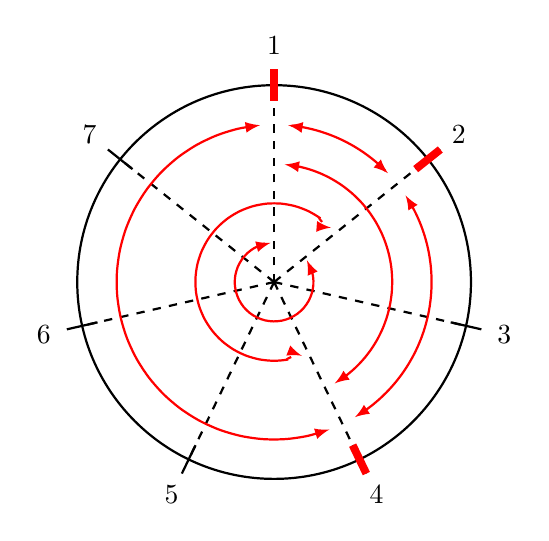
\begin{tikzpicture}
        \def\N{7}
        \draw [thick, black] circle[radius=2.5cm] (0,0);
        \foreach \i in {1,...,\N} {
            \draw [scale=1,domain=2.3:2.7,smooth,variable=\x,black,thick] plot ({\x*sin(360*(\i-1)/\N)},{\x*cos(360*(\i-1)/\N)});
            \draw [black,thick,dashed] (0,0) -- ({2.5*sin(360*(\i-1)/\N)},{2.5*cos(360*(\i-1)/\N)});
            \node[black] at ({3*sin(360*(\i-1)/\N)},{3*cos(360*(\i-1)/\N)}) {$\i$};
        }
        \foreach \i in {0,1,3} {
            \draw [scale=1,domain=2.3:2.7,smooth,variable=\x,red,line width=1mm] plot ({\x*sin(360*\i/\N)},{\x*cos(360*\i/\N)});
        }
        \draw [scale=1,domain=0.1:0.9,smooth,variable=\x,black,thick,>=latex,<->,red] plot ({2*sin(360*\x/\N)},{2*cos(360*\x/\N)}); % 1
        \draw [scale=1,domain=1.1:2.9,smooth,variable=\x,black,thick,>=latex,<->,red] plot ({2*sin(360*\x/\N)},{2*cos(360*\x/\N)}); % 2
        \draw [scale=1,domain=3.1:6.9,smooth,variable=\x,black,thick,>=latex,<->,red] plot ({2*sin(360*\x/\N)},{2*cos(360*\x/\N)}); % 4
        \draw [scale=1,domain=0.1:2.9,smooth,variable=\x,black,thick,>=latex,<->,red] plot ({1.5*sin(360*\x/\N)},{1.5*cos(360*\x/\N)}); % 3
        \draw [scale=1,domain=3.1:7.9,smooth,variable=\x,black,thick,>=latex,<->,red] plot ({1*sin(360*\x/\N)},{1*cos(360*\x/\N)}); % 5
        \draw [scale=1,domain=1.1:6.9,smooth,variable=\x,black,thick,>=latex,<->,red] plot ({0.5*sin(360*\x/\N)},{0.5*cos(360*\x/\N)}); % 6
    \end{tikzpicture}
    \caption{Minimal circular ruler for $N=7$}
    \label{fig:circular-ruler}
\end{figure}

The larger down-sampling factor $N$ with the same $M$ amount of samplers, the better the performance. Finding good solutions for this problem is therefore a convenient optimization for our device. D.Ariananda and G.Leus \todo{ref}, proposed a solution that uses linear sparse ruler to generate solution for the circular sparse ruler problem. The linear sparse ruler problem is identical to the circular sparse ruler, but the only one period is considered. Therefore the ends do not connect, as is illustrated in \cref{tkz:linear_sparse_ruler}.  

\begin{figure}[H]
\centering
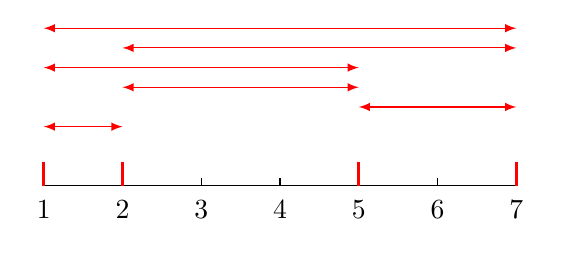
\begin{tikzpicture}

\draw (0,1) -- (6,1);

\draw [red, very thick] (0,1) -- (0,1.3);
\draw [red, very thick](1,1) -- (1,1.3);
\draw (2,1) -- (2,1.1);
\draw (3,1) -- (3,1.1);
\draw [red, very thick](4,1) -- (4,1.3);
\draw (5,1) -- (5,1.1);
\draw [red, very thick](6,1) -- (6,1.3);

\draw [red, >=latex,<->] (0,1.75) -- (1,1.75);
\draw [red, >=latex,<->](4,2) -- (6,2);
\draw [red, >=latex,<->](1,2.25) -- (4,2.25);
\draw [red, >=latex,<->](0,2.5) -- (4,2.5);
\draw [red, >=latex,<->](1,2.75) -- (6,2.75);
\draw [red, >=latex,<->](0,3) -- (6,3);

\node at (0,0.7) {1};
\node at (1,0.7) {2};
\node at (2,0.7) {3};
\node at (3,0.7) {4};
\node at (4,0.7) {5};
\node at (5,0.7) {6};
\node at (6,0.7) {7};

\end{tikzpicture}
\caption{linear sparse ruler with $N=7$ and $M=4$}\label{tkz:linear_sparse_ruler}
\end{figure}

The proposed method in ref\todo{ref} is that a linear sparse solution for $N=x$ is also a circular sparse ruler solution for $N=2(x-1)$ when $x$ is even, and $N=2x-1$ when $x$ is odd. This can be readily seen, because for every lag $L_i<\lfloor\frac{N}{2}\rfloor$, there is also a lag $L_j = N-L_i$. The linear sparse solution in \cref{tkz:linear_sparse_ruler} of $\{1,2,5,7\}$ with $N=7$, is therefore also a circular sparse ruler solution for $N=13$ as is illustrated in \cref{tkz:linear_sparse_ruler}. 

\begin{figure}[H]
\centering
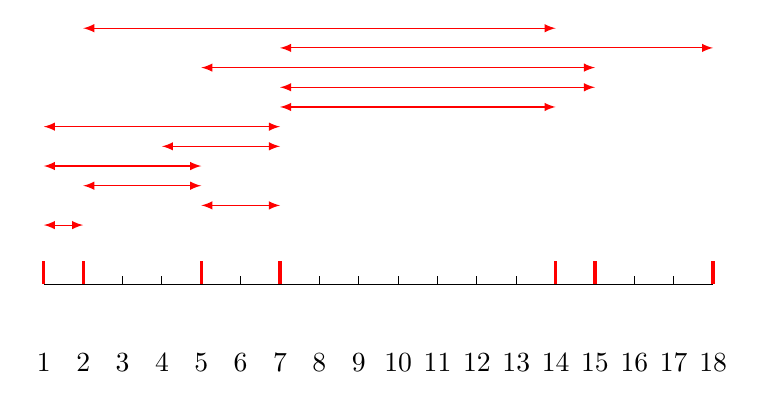
\begin{tikzpicture}

\draw (0,1) -- (8.5,1);

\draw [red, very thick] (0,1) -- (0,1.3);
\draw [red, very thick](.5,1) -- (.5,1.3);
\draw (1,1) -- (1,1.1);
\draw (1.5,1) -- (1.5,1.1);
\draw [red, very thick](2,1) -- (2,1.3);
\draw (2.5,1) -- (2.5,1.1);
\draw [red, very thick](3,1) -- (3,1.3);
\draw  (3.5,1) -- (3.5,1.1);
\draw (4,1) -- (4,1.1);
\draw (4.5,1) -- (4.5,1.1);
\draw (5,1) -- (5,1.1);
\draw (5.5,1) -- (5.5,1.1);
\draw (6,1) -- (6,1.1);

\draw [red, very thick] (6.5,1) -- (6.5,1.3);
\draw [red, very thick](7,1) -- (7,1.3);
\draw (7.5,1) -- (7.5,1.1);
\draw (8,1) -- (8,1.1);
\draw [red, very thick](8.5,1) -- (8.5,1.3);

\draw [red, >=latex,<->] (0,1.75) -- (.5,1.75);
\draw [red, >=latex,<->](2,2) -- (3,2);
\draw [red, >=latex,<->](.5,2.25) -- (2,2.25);
\draw [red, >=latex,<->](0,2.5) -- (2,2.5);
\draw [red, >=latex,<->](1.5,2.75) -- (3,2.75);
\draw [red, >=latex,<->](0,3) -- (3,3);
\draw [red, >=latex,<->](3,3.25) -- (6.5,3.25);
\draw [red, >=latex,<->](3,3.5) -- (7,3.5);
\draw [red, >=latex,<->](2,3.75) -- (7,3.75);
\draw [red, >=latex,<->](3,4) -- (8.5,4);
\draw [red, >=latex,<->](.5,4.25) -- (6.5,4.25);

\node at (0,0) {1};
\node at (.5,0) {2};
\node at (1,0) {3};
\node at (1.5,0) {4};
\node at (2,0) {5};
\node at (2.5,0) {6};
\node at (3,0) {7};
\node at (3.5,0) {8};
\node at (4,0) {9};
\node at (4.5,0) {10};
\node at (5,0) {11};
\node at (5.5,0) {12};
\node at (6,0) {13};
\node at (6.5,0) {14};
\node at (7,0) {15};
\node at (7.5,0) {16};
\node at (8,0) {17};
\node at (8.5,0) {18};

\end{tikzpicture}
\caption{circular sparse solution for $N=13$}\label{tkz:circ_linear_sparse}
\end{figure}

This approach has one main advantage: solutions for linear sparse ruler can be recycled into circular sparse ruler solutions, and better linear sparse ruler solutions will also result in better circular sparse ruler solutions. Because linear sparse ruler is a well known problem, good solutions are easy to come by. However, the solutions generated are not necessarily optimal. There might be situations in which one can do better than with linear sparse ruler solutions. This problem is by no means trivial and requires clever algorithms to calculate.  

\end{document}
